\documentclass[apj]{emulateapj}

\usepackage[intlimits]{amsmath}
\usepackage{amsthm}
\usepackage{amssymb}
\usepackage{cancel} 
\usepackage{graphicx}
\usepackage{mdwlist}
\usepackage{hyperref}
\usepackage{color}
%\citestyle{aa}

\providecommand{\e}[1]{\times10^{#1}}
\providecommand{\units}[1]{\;\mathrm{#1}}
\providecommand{\diff}[2]{\frac{\partial #1}{\partial #2}}
\providecommand{\ddiff}[2]{\frac{\partial^2 #1}{\partial #2^2}}
\providecommand{\tdiff}[2]{\frac{\mathrm{d} #1}{\mathrm{d} #2}}
\providecommand{\infint}[2]{\int\limits_{-\infty}^{\infty}{#1}\;\mathrm{d}#2} 
\providecommand{\MAA}{\text{\AA}}
\providecommand{\abs}[1]{\left| #1 \right|} % for absolute value
\providecommand{\avg}[1]{\left< #1 \right>} % for average
\providecommand{\grad}[1]{\gv{\nabla} #1} % for gradient
\let\divsymb=\div 
\renewcommand{\div}[1]{\gv{\nabla} \cdot #1} % for divergence
\providecommand{\curl}[1]{\gv{\nabla} \times #1} % for curl
\providecommand{\MAA}{\text{\AA}}
\providecommand{\figwidth}{.9\columnwidth}
\newcommand\numberthis{\addtocounter{equation}{1}\tag{\theequation}}
\numberwithin{equation}{section}

\providecommand{\MJ}{\ensuremath{\units{M_J}}}
\providecommand{\RJ}{\ensuremath{\units{R_J}}}
\providecommand{\MS}{\ensuremath{\units{M_\odot}}}
\providecommand{\RS}{\ensuremath{\units{R_\odot}}}

\shorttitle{Detecting Extra-Solar Planets}
\shortauthors{Tom Badran}

\begin{document}

\title{Detecting Extra-Solar Planets}
\author{Tom Badran\altaffilmark{1}}
\email{badrant@cardiff.ac.uk}
\affiliation{Cardiff School of Physics and Astronomy}
\altaffiltext{1}{Cardiff School of Physics and Astronomy, Cardiff University, Queens Buildings, The Parade, Cardiff, Wales, CF24 3AA, UK}
\date{September 2013 to May 2014}

\begin{abstract}
%!TEX root = project.tex
Since 1995 many extra solar planets have been discovered using the transit method. I have shown that it is possible to detect these planets using relatively low powered ground based optical telescopes (<0.5m), even under very poor seeing conditions. I also present an algorithm for analysing images and a computer program implementation of this algorithm, including an automated pipeline for processing a large sequence of images. Using this computer program, it was determined that the dwarf star, Hat P 20, has a planet of radius $(0.91\pm0.14) R_J$.

\end{abstract}

\section{Introduction}
%!TEX root = project.tex
\subsection{Motivations}

Beyond being interesting in the their own right, there are many reasons to look for, and at the properties of exoplanets. Firstly, up until the discovery of the first extra solar planetary system, PSR 1257+ 12 \cite{wolszczan1992planetary}, we were only sure of the existence of planetary bodies in our own solar system. Now we know that our system is not unusual, and it is in fact very common for stars to have many planets of their own \cite{mcarthur2004detection}, and even binary and ternary star systems to have planetary bodies \cite{marcy2002planet}.

Due to the time scales that astronomical phenomena occur on, looking at events such as star and planet formation is impossible over the lifetimes of humans, so instead we have to look at many examples of bodies at varies stages of their life cycles. By looking at planets in other solar systems we can see how they behave across different stages of their evolution, and this can be used to verify our current thinking and models for how solar systems form.

Each planet in our own system has unique and interesting properties too, so by looking elsewhere we can see how common certain characteristics are across the universe, as well as potentially discovering planets with properties completely unlike any in our own solar system.

The favourite motivator is of course the search for life beyond our own. While there is the possibility of some form of life having existed in the past on Mars \cite{mckay1996search} and the possibility of life on some of the outer moons \cite{mckay2005possibilities}, the potential of finding any kind of life, and especially multi-cellular life and even potentially intelligent life is a huge incentive. As techniques for discovering these planets have improved, there have also been observations of Earth sized planets in the so called habitable zone \cite{wordsworth2011gliese}.

\subsection{Methods of Discovery}

\subsubsection{Transit Method}

By observing the flux from a star over period of time, any orbiting planet that passes in front of the star will cause a slight dip in the observed flux. This change in the light curve allows one to calculate the relative sizes of the planet and the star.


Advantages:
\begin{itemize}
    \item Easy to Perform
    \item Can be done at optical wavelengths
\end{itemize}

Disadvantages:
\begin{itemize}
    \item Only works if orbital plane is in line with observer
    \item High false detection rate (REFERENCE)
    \item Poor results for red giant stars (REFERENCE)
\end{itemize}

\subsubsection{Radial Velocity}

\subsubsection{Pulsar timing}

\subsubsection{Gravitational Microlensing}

\subsubsection{Direct Observation}

Model using formulae from \cite{mandel2002analytic}


\section{Model}
%!TEX root = project.tex
\subsection{Uniform Disk}
\begin{figure}
    \centering
    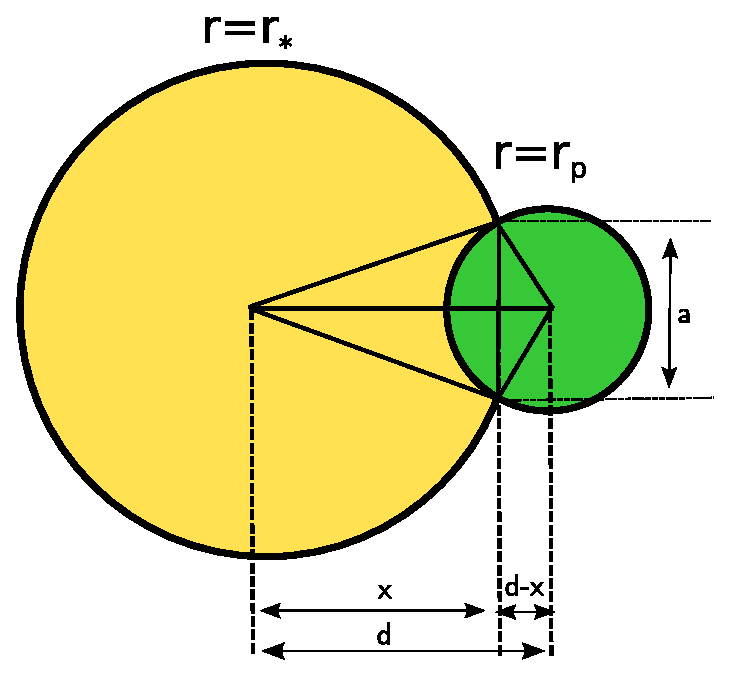
\includegraphics[width=\columnwidth]{images/uniform_disk_overlap.pdf}
    \caption{Overlapping uniform disk model}
    \label{fig:uniform_overlap}
\end{figure}

A very simple model can be made by assuming that the transiting planet is a solid sphere with some radius $r_p$, that blocks all of the radiation from the star. Also, assume that the star itself, with radius $r_*$, emits radiation uniformly from all points, and that it too is a solid sphere.

In this model, there are three positions in the transit that need to be accounted for. Firstly, that the planet disk does not overlap the star, and no radiation is blocked. Secondly, that the planet's disk is fully contained within the disk of the star, and so the emitted radiation is blocked by the complete planetary disk. And thirdly that the disks overlap partially, and some factor less than during a complete overlap is blocked.

The amount of overlap of two circles of different size can be determined as follows:
\begin{align}
    A &= \kappa_1 + \kappa_2 - \kappa_3 \\
    \kappa_1 &= r_p^2\cos^{-1}\left(\frac{d^2 + r_p^2 - r_*^2}{2dr_p}\right)\\
    \kappa_2 &= r_*^2\cos^{-1}\left(\frac{d^2 + r_*^2 - r_p^2}{2dr_*}\right)\\
    \begin{split}
        \kappa_3 &= \frac{1}{2}\sqrt{(-d + r_p + r_*)}\sqrt{(d + r_p - r_*)}\times\\
        &\;\;\;\;\;\;\;\sqrt{(d - r_p + r_*)}\sqrt{(d + r_p + r_*)}
    \end{split}
\end{align}
While I arrived at this model independently, it is mathematically identical to the uniform disk model presented in \cite{mandel2002analytic}, although presented in a different form. An example transit using this model can be seen in figure \ref{fig:uniform_disk_model}. In each model I use a theoretical hot Jupiter, with parameters as shown in table \ref{tab:model}.
\begin{table}
\begin{tabular}{lr}
Star Radius & \RS \\
Star Mass &  \MS \\
Planet Radius & \RJ \\
Planet Mass & $2\MJ$ \\
Separation & $0.2\units{au}$ \\
\end{tabular}
\caption{Table of model parameters}
\label{tab:model}
\end{table}

\begin{figure}
    \centering
    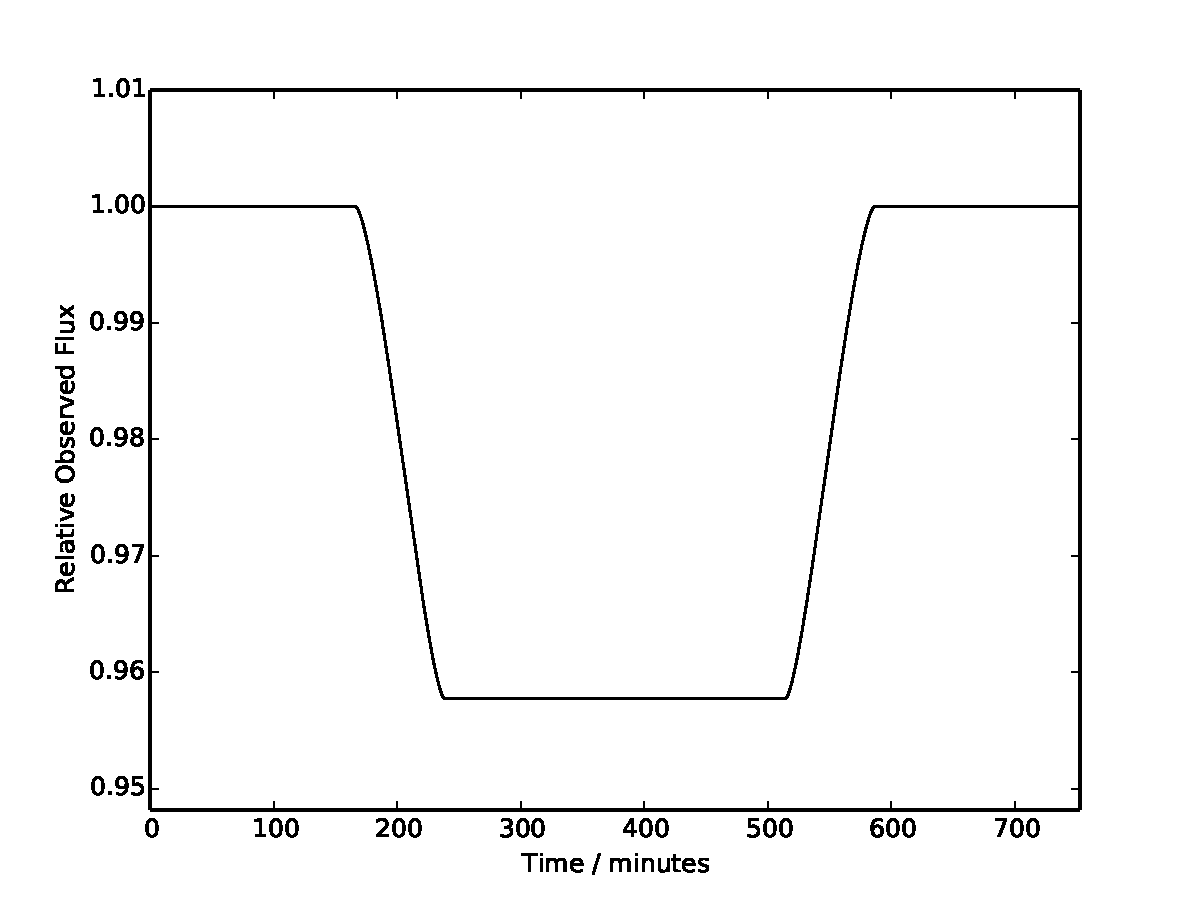
\includegraphics[width=\columnwidth]{images/uniform_disk_model.pdf}
    \caption{Expected observed flux from a transit as modelled as uniform disks}
    \label{fig:uniform_disk_model}
\end{figure}

\subsection{Limb Darkening}

While the uniform disk model is a good approximation, it is not an accurate description of what is observed. Stars appear to in fact have a decreasing intensity towards the outer edge than in the center. This limb darkening is due to two effects. Both the temperature and density of the star decrease as a function of radius. This can be seen clearly in figure \ref{fig:limb_darkening_image}.

\begin{figure}
    \centering
    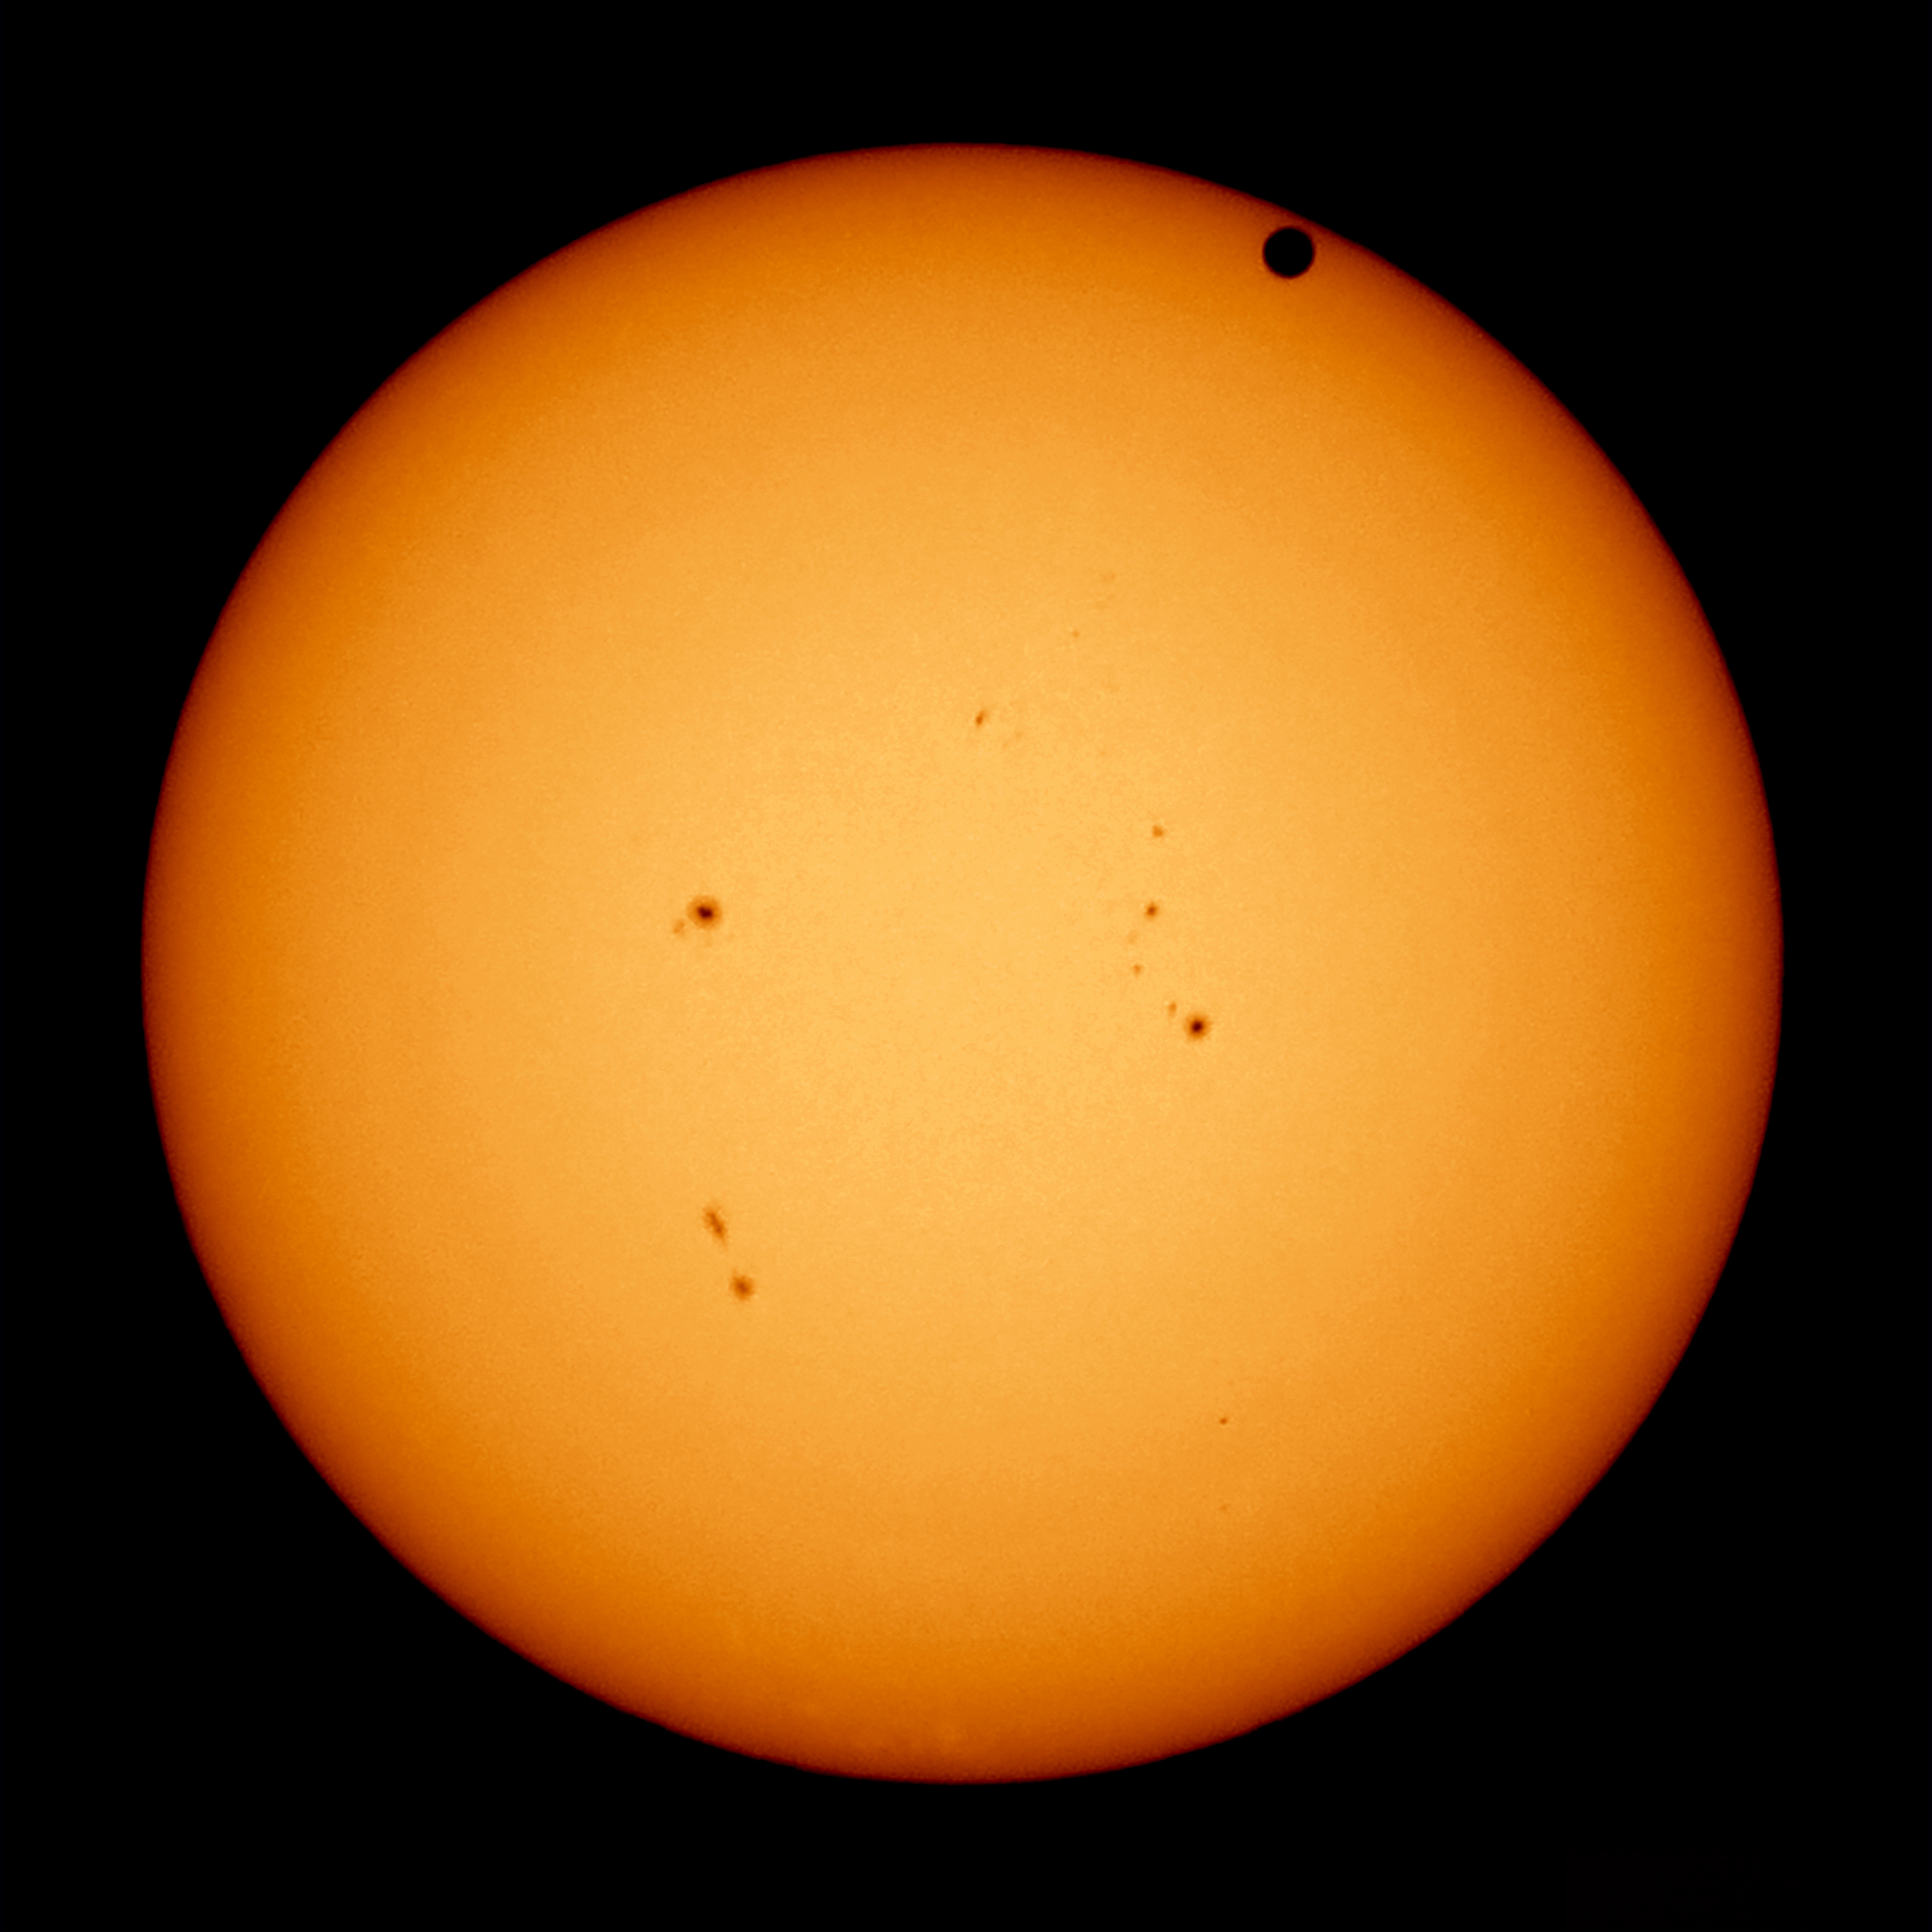
\includegraphics[width=\columnwidth]{images/venus_transit.jpg}
    \caption{Image of the Sun taken during the 2012 Venus Transit, provided courtesy of Brocken Inaglory}
    \label{fig:limb_darkening_image}
\end{figure}

\begin{figure}
    \centering
    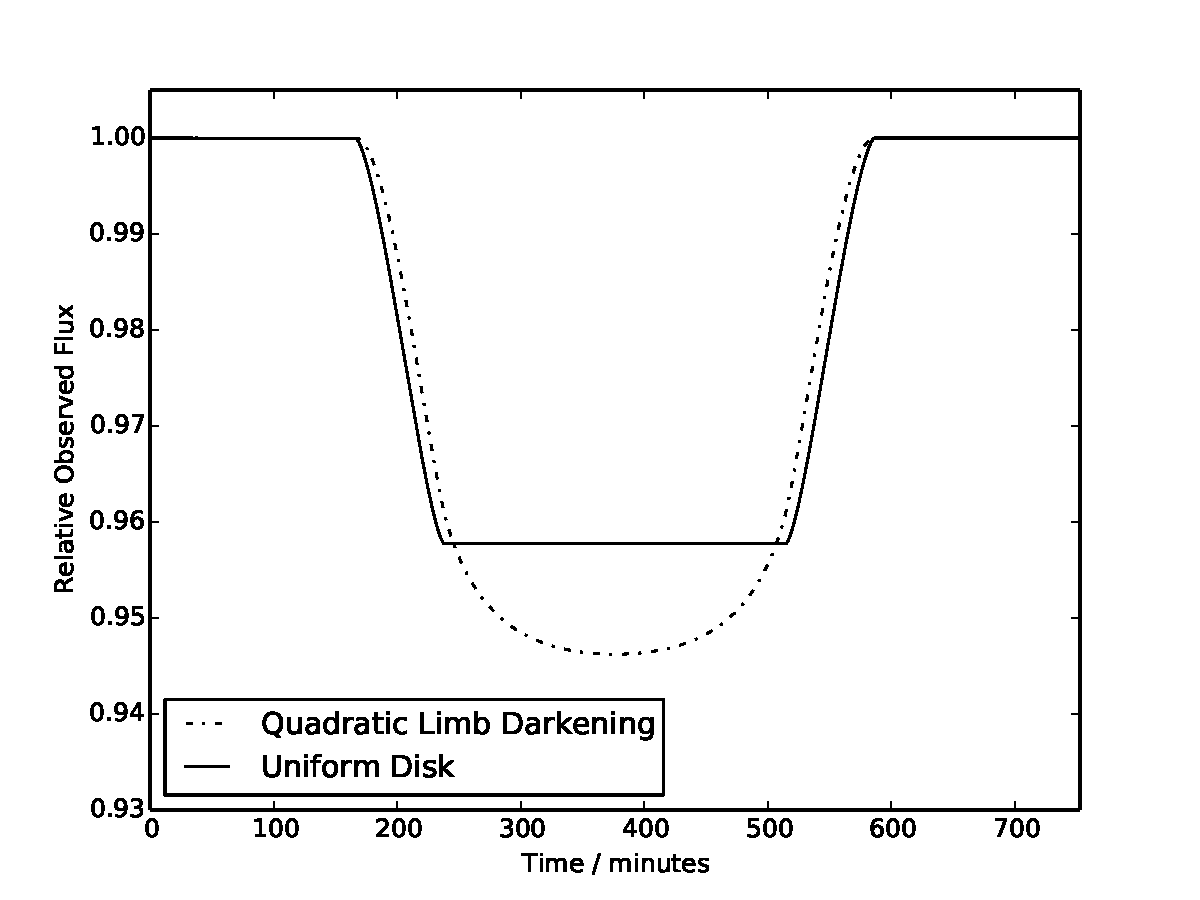
\includegraphics[width=\columnwidth]{images/model_comparison.pdf}
    \caption{Comparison of Uniform disk and quadratic limb-darkening models}
    \label{fig:model_comparison}
\end{figure}


%\bibliographystyle{apj}
\bibliography{references}

\end{document}
